\section{Social Authentication}
\subsection{Introduction}
Social login is a form of single sign-on using existing information from a social networking service such as Facebook, Twitter or Google+, to sign into a third party website instead of creating a new login account specifically for that website.
Our mode of authentication is using the Google login.
\subsection{Features}
\begin{itemize}
	\item As almost every coder has Google account, he/she can easily sign in with Google without any signup.
	\item If we have to conduct a competition within the institute, we can put the filter which will allow only sign in with institute’s email-id.
	\item It saves database memory for storing credentials of the users.
	\item No need to send confirmation mail, and the email would be validated.

\end{itemize}
\subsection{Implementation}
We are using Django Social Auth library to implement this, it is an easy way to setup social authentication/authorization mechanism for Django projects. It provides user login using social websites credentials. It populates data from the social websites and creates new users.

We have a one-one relationship between a user and profile, extra application dependent information is stored in the profile model.


\section{Rich Text Integration}
\subsection{Introduction}
This module aims to integrate a rich text editor with the text field of a form, especially for problem statements and posts. This module can be integrated with either a markdown editor or a WYSIWYG (what you see is what you get) editor. Websites like hackerrank or stackoverflow use a markdown editor, since it is more customizable for people familiar with markdown.
\subsubsection{Markdown Editor}
Markdown is a lightweight markup language with plain text formatting syntax. It can be converted to HTML and many other formats. Markdown is often used to format readme files, for writing messages in online discussion forums, and to create rich text using a plain text editor.
\subsubsection{WYSIWYG Editor}
WYSIWYG implies a user interface that allows the user to view something very similar to the end result while the document is being created. In general, WYSIWYG implies the ability to directly manipulate the layout of a document without having to type or remember names of layout commands.
\begin{figure}[h!]
    \centering
    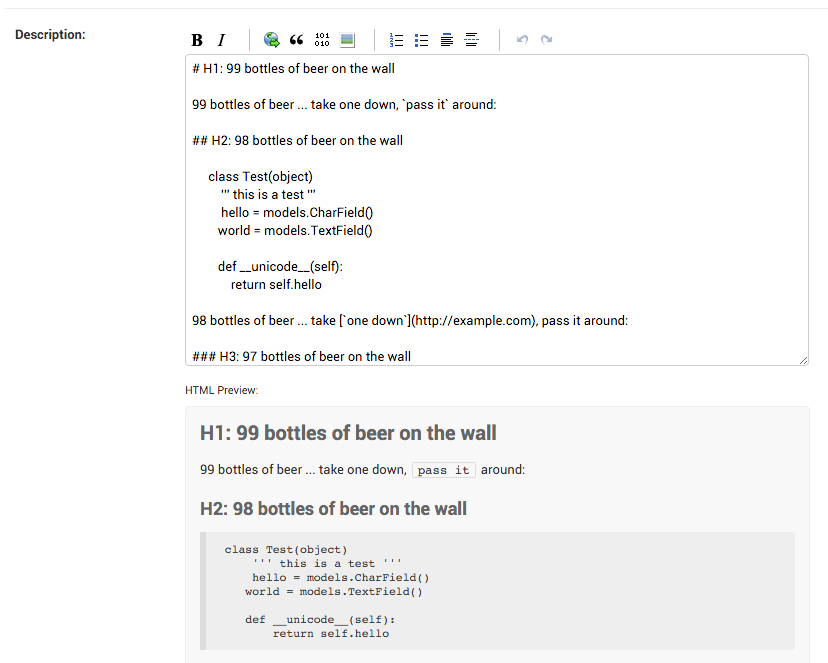
\includegraphics[width=\linewidth]{markdown.png}
    \caption{Example of Markdown Editor}
    \label{fig:markdown}
\end{figure}
\subsection{Use}
The major use for this module to increase readability and writability in text fields like problem statement, contest description, post content, etc.
\subsection{Implementation}
There are several libraries compatible with Django for markdown editing (pagedown) as well as WYSIWYG (tinymce). This libraries allow addition of rich text editors in form fields.

